\chapter{Background}
\label{Chapter2}
% Main chapter title
\lhead{Chapter 2. \emph{Background}}


This chapter introduces the background necessary to understand the concepts and methods presented in this thesis. Different sections throughout this chapter will deal with important terminologies that are essential for the foundation of this research. 
% Important terminologies essential for the foundation of this thesis are explained in subsequent sections throughout this chapter.

%  it is beneficial to test the important functional use-cases on the AUT through this layer. 
Section \ref{sec:AutomatedGUITesting} gives a brief insight into the automated GUI testing mechanisms since a majority of web applications' functionality is accessed through the GUI layer. Moreover, this section discusses the challenges of GUI testing with existing automated testing approaches. 

As Selenium \cite{websiteSelenium} has been a popular browser test automation tool among software developers and testers in recent years, Section \ref{sec:SeleniumTesting} provides the necessary background about its implementation techniques as well as salient features.

This thesis utilizes existing Selenium tests to capture the behavior of the AUT in terms of behavioral state models, as mentioned in Chapter \ref{Chapter1}. For this purpose, the tool \texttt{webmate} presented by Dallmeier et al. \cite{webmate} has been used. By leveraging existing Selenium tests, \texttt{webmate} can systematically explore the AUT to extract its behavioral usage-model. Further details about \texttt{webmate} are, therefore, discussed in Section \ref{sec:WebMate}.

Section \ref{sec:Statistical} elaborates the statistical background required to analyze the results and apply the evaluation metrics, as presented in Chapter \ref{Chapter3}, while Section \ref{sec:relatedWork} discusses the state-of-the-art in automated testing and provides the literature review about important research publications directly or indirectly related to the research presented in this thesis. 

\section{Automated GUI Testing}
\label{sec:AutomatedGUITesting}
As mentioned in Chapter \ref{Chapter1}, testing web applications at GUI level abstracts away finer grained internal details and helps developers to identify the undesired functionality changes in the AUT. In comparison to traditional command-line applications, automated GUI testing of modern web 2.0 applications built with multiple languages, platforms and server-side technologies poses new challenges.

First and foremost, automatically generating and selecting inputs for a GUI is difficult since different applications might require specific combinations of inputs and values. 
Current practices for automated test input generation include techniques such as symbolic execution \cite{Ganovetal}, using random input generation \cite{godefroid2005dart} or search based techniques \cite{gross2012search}. Nevertheless, automated input generation is not trivial for a web application, since the GUI test automation tool needs to be aware of the context of the AUT. Thus, in many cases, input generation is often left to the test developer to explore the desired states of the AUT hidden behind input forms and elements.

Secondly, even in cases when a testing tool can generate different input combinations automatically, it still needs to verify the correct behavior of the AUT. This is usually done by applying appropriate test assertions and oracles on the test outputs \cite{Baresi:Oracles}. The capture/replay tools \cite{joshi2006capture} require the tester to first manually capture the behavior of the AUT by performing different GUI-level events and recording the output. In the replay phase, recorded tests are replayed on the AUT and the output is checked against the captured \textit{expected output} for asserting the application behavior. This requires manual effort to record each test and is not suitable for regression testing as every time the AUT changes \cite{sjosten2006costs}, \cite{leotta2013capture}, there is a need of re-recording the tests in order to generate new expected outputs. 

Moreover, as the size of the AUT increases, the number of possible actions on the GUI increases as well. This leads to the fact that covering the entire possible number of state space becomes infeasible. In comparison to automated testing tools, such as crawlers and test generators, humans possess the domain knowledge of the AUT required to generate valid test inputs and apply precise oracles on the test outputs. Thus, many developers often choose to identify the core functionality of the AUT and automate their regression tests using frameworks such as Selenium \cite{websiteSelenium}, as detailed in Section \ref{sec:SeleniumTesting}.

\section{Test Automation with Selenium}
\label{sec:SeleniumTesting}
\subsection{Architecture}
\label{ssec:webdriverArchitecture}
Selenium is a browser automation framework designed to automate the system testing of web applications. While the Selenium project offers a different set of tools depending upon the type of application, the  \texttt{webdriver}\footnote{\url{http://www.seleniumhq.org/projects/webdriver/}} based tests are the focus of this thesis. The \texttt{webdriver} project provides an API to test dynamic web 2.0 applications. 

The \texttt{webdriver} API supports various modern programming languages such as Java, Python, C\#, Ruby, PHP, etc. by providing language level bindings along with a set of browser specific drivers. Figure \ref{fig:webdriverArchitecture} gives an overview of the architecture of Selenium \texttt{webdriver}.

The API \textit{drives} (controls) the browser in a manner that it emulates all possible end users interactions with the browser, such as clicks, form-inputs, drag-drops, file uploads, etc. Selenium \texttt{webdriver} tests can thus explore the possible set of functionalities of the AUT. As an example, Snippet \ref{code1} illustrates a \texttt{webdriver} test case (Java) to test the \textit{login} functionality of AUT as depicted in Figure \ref{fig:a}.
\begin{center}
\begin{scriptsize}
\centering
\lstset{
  basicstyle=\ttfamily,
  columns=fullflexible,
  keepspaces=true,
%   frame=none,
}
% \verb|basicstyle=\ttfamily, columns=fullflexible, keepspaces=true|
  
\begin{lstlisting}[caption=Login test,label=code1]
public void loginTest(){
driver.get("http://www.application-under-test.com");
driver.findElement(By.id("uname")).sendKeys("user");
driver.findElement(By.id("pwd")).sendKeys("passwd");
driver.findElement(By.linkText("Login")).click();
}
\end{lstlisting}
\end{scriptsize} 
\end{center}
 
\begin{figure}[h! ]
\makeatletter 
% \renewcommand{\thefigure}{\@arabic\c@figure}
\makeatother
    \centering
  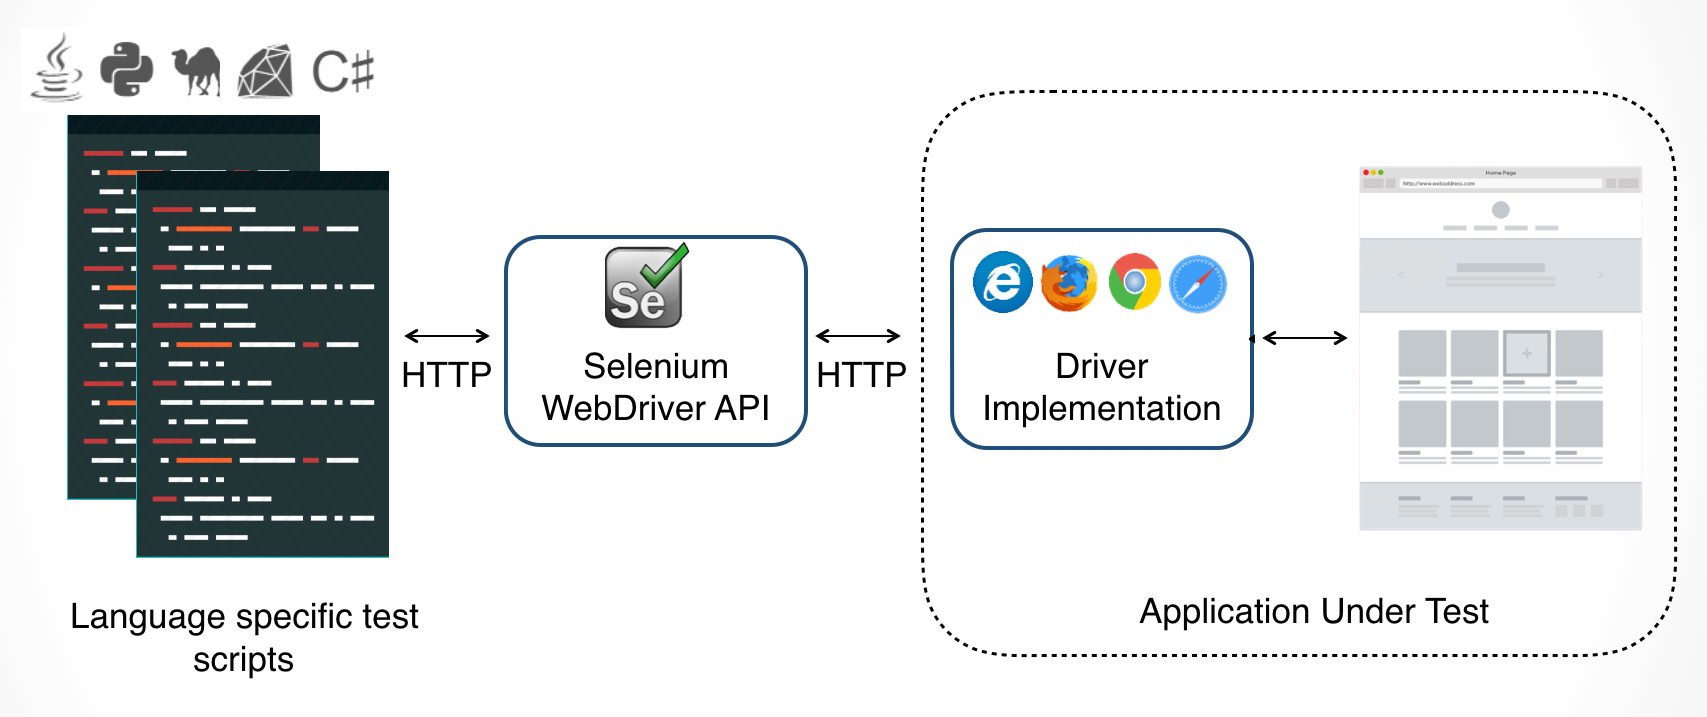
\includegraphics[width=5.5in,height=2.2in]{./Figures/webdriver_Archi}
  \caption{Selenium \texttt{webdriver} architecture}
  \label{fig:webdriverArchitecture} 
\end{figure}

The \texttt{webdriver} API communicates with the browser specific driver using a common wire protocol. The protocol transfers the test commands written in language specific bindings to the browser specific driver in the form of UTF-8\footnote{\url{https://tools.ietf.org/html/rfc3629}} encoded JSON\footnote{\url{http://www.json.org/}} data. The API uses HTTP\footnote{\url{https://www.w3.org/Protocols/}} as a transport mechanism to transfer these commands to the driver and to return the response from the driver to the language specific code. 
\noindent 
The following example illustrates the communication between the language specific test commands (Java in this case) and the \texttt{RemoteWebDriver} through \texttt{webdriver} API :
\begin{enumerate}
\item The client (test script) requests the URL of the AUT.\\
\begin{small}
\texttt{driver.get("http://www.application-under-test.com");}
\end{small}
\item This command is translated as a JSON object to be transferred using the wire protocol as following:\\
\begin{small}
\texttt{\{"url": "http://www.application-under-test.com"\}}
\end{small}
\item The JSON object is then sent over HTTP (using POST\footnote{\url{http://tools.ietf.org/html/rfc7231\#section-4.3.3}} request in this case). To identify and associate each request/response session uniquely to the session-specific commands, \texttt{webdriver} uses a unique handle in terms of the \textit{SessionId}\footnote{\url{https://w3c.github.io/webdriver/webdriver-spec.html\#sessions}}\\
\begin{small}
\texttt{Method : POST, Path: session/{session-id}/url}\\
\end{small}
The resultant URL is :\\
\begin{small}
\texttt{http://localhost:7055/hub/session/{session-id}/url}
\end{small}
\end{enumerate}

Each browser specific driver implementation, such as the \texttt{Firefox Driver} or the \texttt{RemoteWebDriver}, has its own mechanism for carrying out the above-mentioned communication. 

The \texttt{RemoteWebDriver} implementation provides the capability to run the Selenium tests against a remote machine. In essence, \texttt{RemoteWebDriver} is comprised of a client-server architecture, where client is the language specific test-case and and server is a simple Java servlet. The \texttt{RemoteWebDriver} servlet acts as a multiplexer, by connecting the client to the specific browser(s) and system configurations requested by the client. The browser and other configurations are provided in terms of capabilities, via command-line or directly from the language specific code.
\subsection{Test Design and Composition}
\label{testDesignPractices}
As illustrated in Section \ref{ssec:webdriverArchitecture}, a Selenium test can emulate various user-actions on AUT. In order to do so, a test needs to perform various steps such as navigating to the AUT, locating the GUI elements and finally performing these user-actions. This section gives an overview about the basic building blocks of a Selenium test. 
\subsubsection{Locating GUI Elements}
\label{sssec:locatingUIElements}
In order to locate GUI elements such as input forms, buttons, checkboxes, etc. in the DOM (Document Object Model), \texttt{webdriver} specifies \textit{``Find Element''} and \textit{``Find Elements''} methods for locating a single element and a list of elements, respectively. 
Within the scope of these methods, it is also possible to traverse the DOM tree to locate the \textit{Child Elements}, i.e. children nodes of a parent element in the tree. 
Each language specific binding has its own command to invoke these methods by providing the GUI element locator object, such as\begin{small} HTML\end{small} \texttt{id}, the \texttt{css selector} or \texttt{xpath} expressions.

% \begin{verbatim}
% % \#Classification : STRUCTURAL VS NON-STRUCTURAL
% % \#ADVANTAGE/PROPERTIES IN SHORT
% % \#IMPLEMENTATION EXAMPLE,
% \end{verbatim}

The most commonly  used\footnote{\url{http://www.seleniumhq.org/docs/03_webdriver.jsp\#locating-ui-elements-webelements}} GUI locators and their implementation in Java is listed as following:
\begin{itemize}
% ### ID
\item 
By \texttt{id}:
Locates the GUI element using \texttt{id} attribute of \begin{footnotesize} HTML\end{footnotesize} element.
\newline
\begin{footnotesize}
\framecolorbox[\linewidth][l]{gray}{white}{\texttt{<input id="login" type="button"/>}}
\texttt{WebElement loginButton = driver.findElement(By.id("login"));
}
\end{footnotesize}
% Locating UI Elements using unique HTML \texttt{id} attributes is the most preferred and reliable method\footnote{\url{http://www.seleniumhq.org/docs/03_webdriver.jsp\#by-id}}.  
% #NAME
\item 
By \texttt{name}:
Locates the GUI element using \texttt{name} attribute of \begin{footnotesize} HTML\end{footnotesize} element.
\newline
\begin{footnotesize}
\framecolorbox[\linewidth][l]{gray}{white}{\texttt{<input type="button" name="login"/>
}}
\texttt{WebElement loginButton = driver.findElement(By.name("login"));
}
\end{footnotesize}
% #Class name
\item 
By \texttt{class name}:
Locates the GUI element using the value of \begin{footnotesize} HTML\end{footnotesize} \texttt{class} attribute.
\newline
\begin{footnotesize}
\framecolorbox[\linewidth][l]{gray}{white}{\texttt{<input type="button" class="login"/>
}}
\texttt{WebElement loginButton = driver.findElement(By.className("login"));
}
\end{footnotesize}

% #tag name
\item 
By \texttt{tag name}:
Locates the GUI element using the \begin{footnotesize} HTML\end{footnotesize} \texttt{tag} attribute.
\newline
\begin{footnotesize}
\framecolorbox[\linewidth][l]{gray}{white}{\texttt{<button name="login"</button>
}}
\texttt{WebElement loginButton = driver.findElement(By.tagName("button"));
}
\end{footnotesize}

% #link text
\item 
By \texttt{link text}:
Locates the GUI element using the visible text of the hyperlink.
\newline
\begin{footnotesize}
\framecolorbox[\linewidth][l]{gray}{white}{\texttt{<a href="\#">Login</a>}}
\texttt{WebElement loginButton = driver.findElement(By.linkText("Login"));
}
\end{footnotesize}

% # partial link text
\item 
By \texttt{partial link text}:
Locates the GUI element by partial matching of visible text of the hyperlink.
\newline
\begin{footnotesize}
\framecolorbox[\linewidth][l]{gray}{white}{\texttt{<a href="\#">Login Here</a>}}
\texttt{WebElement loginButton = driver.findElement(By.partialLinkText("Login"));
}
\end{footnotesize}
% # CSS
\item 
By \texttt{css selector}:
Locates the GUI element using the \texttt{css selector} representing the \begin{footnotesize} HTML\end{footnotesize} \texttt{tags, name, class and id} attributes through various combinations.\texttt{css selectors} also allow locating parent and children nodes of a DOM tree. 
\newline
\begin{footnotesize}
\framecolorbox[\linewidth][l]{gray}{white}{\texttt{<input id="login"/>
}}
\texttt{WebElement loginButton = driver.findElement(By.cssSelector("input\#login"));
}
\end{footnotesize}
% # xpath
\item 
By \texttt{xpath}:
Locates the GUI element using the \texttt{xpath} expressions as it supports navigating XML as well as xHTML element tree. Similar to \texttt{css selectors}, the \texttt{xpath} expressions also allow locating parent and children nodes of a DOM tree. 
\newline
\begin{footnotesize}
\framecolorbox[\linewidth][l]{gray}{white}{\texttt{<input id="login"/>
}}
\texttt{WebElement loginButton = driver.findElement(By.xpath("//input[@id="login"]"));
}
\end{footnotesize}
\end{itemize}
Depending upon the GUI structure of AUT and the applicability of GUI element locators, different location strategies can be used in combination. The Influence of these GUI locator strategies on the robustness of Selenium tests is discussed in Chapter \ref{Chapter3}.
% (https://w3c.github.io/webdriver/webdriver-spec.html#sessions)
\subsubsection{Emulating User Actions}
\label{sssec:emulatingActions}
Upon locating the desired GUI element, \texttt{webdriver} API allows us to emulate various user actions on it depending on the element type. These actions can be classified into \textit{state-changing actions}, assertions and requesting additional information about the AUT, such as cookies. A state-changing action signifies a change in the DOM state of the AUT. The most common ways are to emulate the mouse and keyboard based actions by the user, such as clicking (e.g. \texttt{click} element) and form-filling (e.g. \texttt{SendKeys} to element). Moreover, the API makes it possible to perform assertions on the AUT supported by native language scripts such as getting the title or heading of the web page to ensure that correct page has been navigated. 

State changing actions trigger a change the GUI state of the application. Such change does not necessarily navigate the user to another web page, but nonetheless change the contents or the information of the AUT at a given instant.

\subsubsection{Using Wait Conditions}
\label{sssec:seleniumwaits}
The Selenium \texttt{webdriver} API provides the possibility to introduce \textit{wait} conditions in the tests when the test needs to wait for a response from the AUT. These commands can instruct the \texttt{webdriver} to wait after loading a page or before locating a GUI element. The wait commands can be classified as implicit and explicit wait commands. 

When locating an element in the DOM, implicit wait tells the \texttt{webdriver} to wait for a certain amount of time while locating an element. If the element is not found, \texttt{webdriver} waits for the amount of time specified by the implicit wait before throwing an exception, such as \texttt{NoSuchElementException}. Implicit waits can be defined in the setup methods of the tests and are set for the entire duration of the browser session. Following example shows the usage of implicit wait:
\begin{small}
\texttt{ driver.manage().timeouts().implicitlyWait(5, TimeUnit.SECONDS); 
}
\end{small}

Explicit waits specify the test to wait until certain condition is satisfied. In comparison to implicit waits where the test halts for the specified time duration, test with explicit wait proceeds the next step of the test as soon as the expected condition is met. By default, the explicit wait condition is checked every 500 milliseconds. If the element is not found within the specified duration, exception such as \texttt{TimeoutException} is thrown. In the following example, the test would click the ``Login'' button as soon as the \texttt{webdriver} finds that the element is clickable.
\begin{small}
\begin{verbatim}
WebDriverWait wait = new WebDriverWait(driver, 10);
WebElement element = wait.until(ExpectedConditions.
                     elementToBeClickable(By.linkText("Login"))));
\end{verbatim}
\end{small}

\subsubsection{Page-Object Pattern}
\label{page-object}
Since its inception, the page-object design pattern\footnote{\url{http://www.seleniumhq.org/docs/06_test_design_considerations.jsp\#page-object-design-pattern}} has been a widely used standard for designing Selenium \texttt{webdriver} tests. 
Page-object pattern encapsulates pages of an application as a series of objects and essentially provides a logical coupling between the test code and the page-object specific code, such as the GUI locators. Such a design pattern reduces code duplication and improves readability of tests. The test in Listing \ref{code1} can be designed using the page-object pattern as following: 

\begin{center}
\begin{scriptsize}
\centering
\lstset{
  basicstyle=\ttfamily,
  columns=fullflexible,
  keepspaces=true,
%   frame=none,
}
% \verb|basicstyle=\ttfamily, columns=fullflexible, keepspaces=true|
  
\begin{lstlisting}[caption=Page-Objects design for \texttt{loginTest},label=code2]
// Page-objects (POs)
public class HomePage(){ // home page PO
Webdriver driver;
public HomePage(WebDriver driver){
this.driver=driver;
}}

public class LoginPage(){ // login page PO
Webdriver driver;
public static final By uname = By.id("uname");
public static final By pwd = By.id("pwd");
public static final By loginButton = By.linkText("Login");

public LoginPage(WebDriver driver){this.driver=driver;}
public HomePage peformLogin(String user,String pwd){
driver.findElement(uname).sendKeys(user);
driver.findElement(pwd).sendKeys(pwd);
driver.findElement(loginButton).click();
return new HomePage(driver)
}}

@Test // loginTest test
public void loginTest(){
WebDriver driver;
LoginPage loginPage = new LoginPage(driver);
HomePage homePage = loginPage.performLogin("uname","passwd");
}}
\end{lstlisting}
\end{scriptsize} 
\end{center}
 
As illustrated in Listing \ref{code2}, the page-object pattern allows us to model the GUI in the test cases in an object-oriented manner. Although such an approach seems verbose at first, it helps to reduce the possible duplication of the test code. As an example, in situations when user login is to be performed multiple times, which is typically required for many websites performing user validation, page-object backed \texttt{loginTest} serves a more modular implementation. 

Moreover, page-object pattern contributes towards the maintainability and robustness of tests \cite{leottaPObs}, as mentioned in Chapter \ref{Chapter3}.


\section{WebMate}
\label{sec:WebMate}
As mentioned in Chapter \ref{Chapter1}, \texttt{webmate} \cite{webmate} is a system-level automated testing and analysis framework. Primarily developed as a cross-browser compatibility testing tool, \texttt{webmate} supports different browsers and platforms. It can leverage existing Selenium tests in order to remote control the browser to interact with the dynamic web 2.0 applications involving JavaScript and Ajax elements. 

By leveraging the Selenium tests, \texttt{webmate} explores the AUT and extracts a \textit{usage-model}. The usage-model represents a finite state model which captures various actions performed by the Selenium test on the AUT. The states of the usage-model correspond to different states of the GUI and the transitions correspond to different interactions with the AUT such as clicks, form-inputs, etc. For each state of the usage-model, \texttt{webmate} is able to record its visual (GUI) state, in the form of a screen-shot of the AUT.

Figure \ref{fig:webmateArchitecture} gives an example of \texttt{webmate} to leverage the \texttt{loginTest} (see Listing \ref{code1}) to generate the usage-model. In this example, the states of the model represent the DOM states of the AUT and edges represent \textit{actions} executed by the test, such as a \textit{click} action. For security reasons, Selenium tests are integrated with \texttt{webmate} inside a virtual machine. The virtual machine hosts a Selenium hub\footnote{\url{http://www.seleniumhq.org/docs/07_selenium_grid.jsp}} infrastructure, along with a set of browsers. Existing Selenium tests are executed with \texttt{webmate} by using the \texttt{RemoteWebDriver} capabilities, such as specifying browser name, security credentials for \texttt{webmate} etc. The usage-models are generated by \texttt{webmate} without interfering with the underlying Selenium tests. 

Using \texttt{webmate} it is possible to recognize functional differences (e.g. missing button) by comparing the usage-models. As we will see in Chapter \ref{Chapter3}, this comparison is essential for our analysis and \texttt{webmate} fits our requirement of a testing tool which can leverage existing Selenium tests to capture test execution in terms of behavioral state models. Therefore, \texttt{webmate} is used as a tool of choice in this thesis for establishing the ground truth for the robustness analysis, as detailed in Chapter \ref{Chapter6}.

\begin{figure}
\makeatletter 
% \renewcommand{\thefigure}{\@arabic\c@figure}
\makeatother
    \centering
  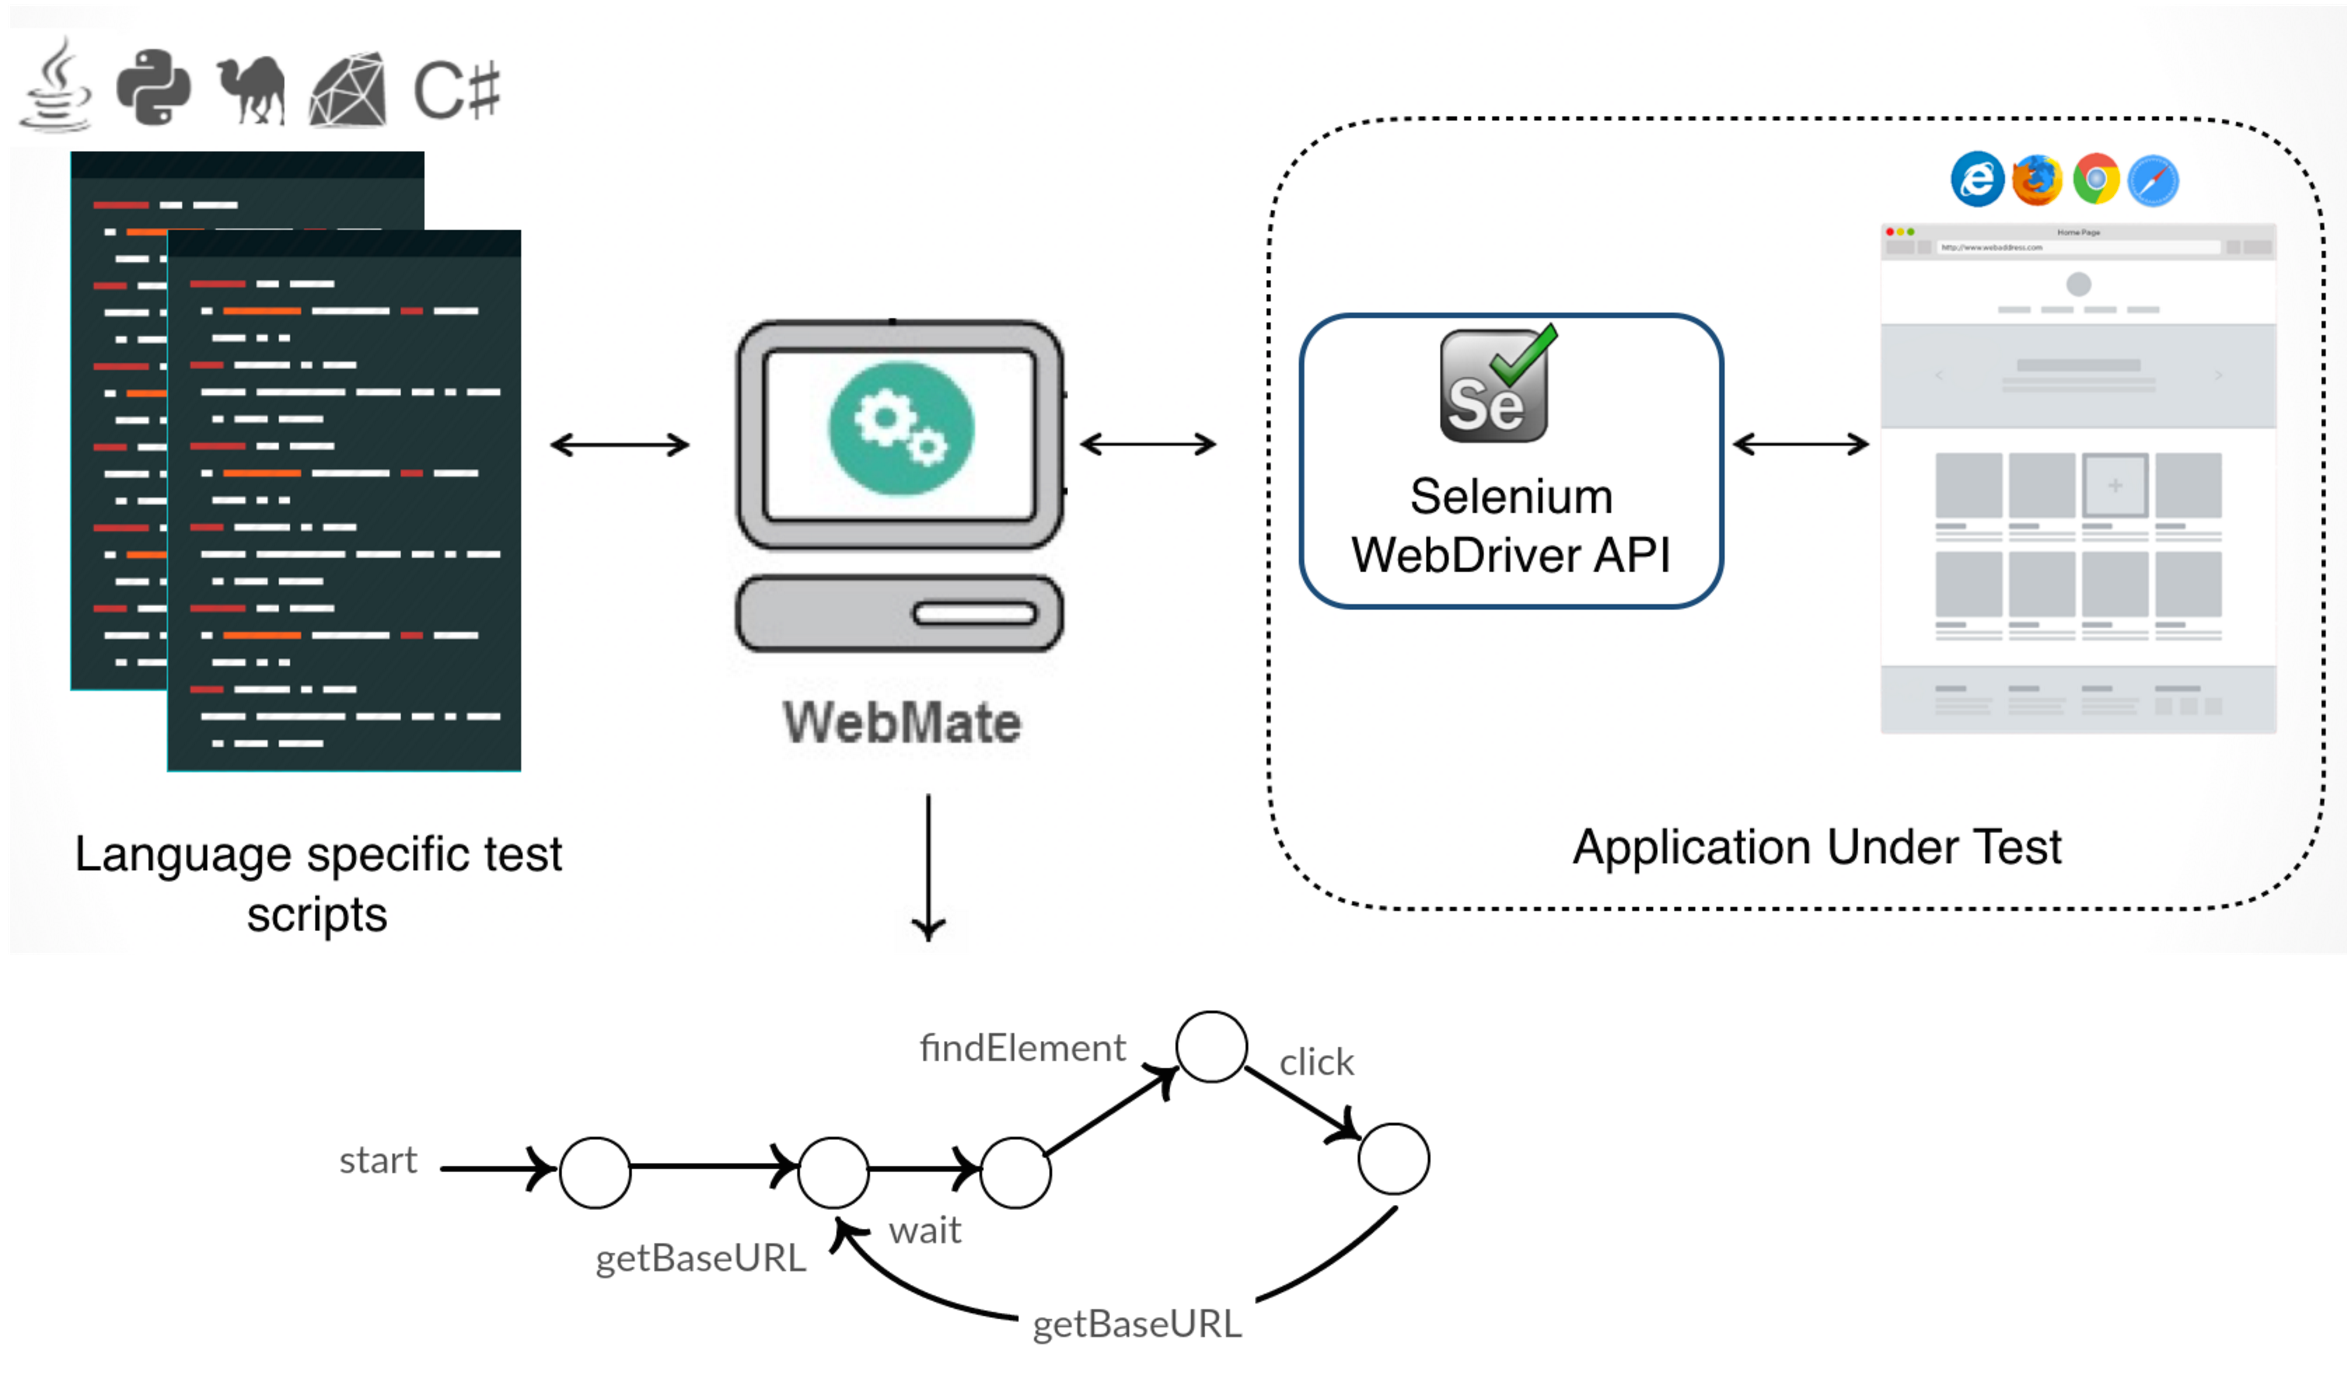
\includegraphics[width=5.5in,height=3in]{./Figures/webmate-state-graph}
  \caption{Webmate architecture}
  \label{fig:webmateArchitecture} 
\end{figure}


% \begin{figure}
% \makeatletter 
% \renewcommand{\thefigure}{\@arabic\c@figure}
% \makeatother
% % \setcounter{figure}{0}
%     \centering
%   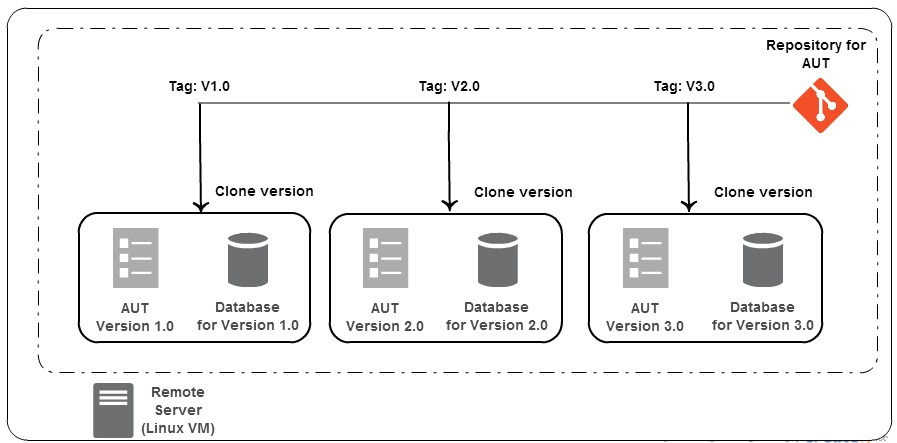
\includegraphics[width=5.4in,height=2.6in]{./Figures/Deployment_Process_2.jpg}
%   \caption{Automatic parallel deployment process}
%   \label{fig:deployment} 
% \end{figure}

\section{Statistical Background}
\label{sec:Statistical}
Adhering to the goals of this thesis, the metrics influencing the robustness of Selenium tests have been developed in Chapter \ref{Chapter3}. To identify which metrics impact the robustness of Selenium tests the most, it is important to statistically evaluate the significance of these metrics. This section presents the statistical background and terminology necessary for this evaluation.

For the statistical analysis, the robustness metrics are represented in by an $i\times j$  \textit{feature matrix} \cite{li2005lasso}. Each of the \textit{j} columns of the feature matrix represents a robustness metric, and each row
\textit{i} represents a Selenium tests. To assess the influence each metric has on robustness, the feature matrix is annexed by a \textit{solution vector} column as depicted in Figure \ref{fig:featurematrix}. A \textit{solution vector} is the ground truth established by executing Selenium tests with the \texttt{webmate} setup, as mentioned in Section \ref{sec:WebMate}.

\begin{figure}[ht]
\[
Feature\smallskip Matrix_{i,j} = 
\begin{pmatrix}
  a_{1,1} & a_{1,2} & \cdots & a_{1,j} & | & \textit{$sv_{1}$}\\
  a_{2,1} & a_{2,2} & \cdots & a_{2,j} & | & \textit{$sv_{2}$}\\
  \vdots  & \vdots  & \ddots & \vdots  & \vdots & \vdots \\
  a_{i,1} & a_{i,2} & \cdots & a_{i,j} & | & \textit{$sv_{i}$}
\end{pmatrix}
\]
\caption{Feature Matrix with Solution Vector}
\label{fig:featurematrix}
\end{figure}

\subsection{Correlation}
It would be interesting to know which of the presented metrics has the highest influence on the robustness of Selenium tests. The term \textit{`correlation'} indicates a statistical relationship between two experimental variables. It is important to note that \textit{`correlation'} does not necessarily imply causation. For the  purpose of statistical evaluation of this thesis, \textit{rank correlation} is a suitable method for estimating the correlation between the features (robustness metrics) and the solution vector (ground truth).

We use \textit{Spearman rank correlation} as the method for estimating correlation (see Definition \ref{def:spearman}). This definition is also applicable in case of \textit{ties} in the ranks of independent variables. For estimating the Spearman's correlation coefficient between two variables, a monotonic relationship is sufficient. The value of Spearman's correlation coefficient falls in the range [-1,1]. A high positive correlation coefficient (approaching ``1'') indicates that when value of one experimental variable increases, value of other variable increases as well. On the other hand, a high negative value (approaching ``-1'') indicates that when value of one variable increases, value of other variable decreases. Whereas a value close to zero indicates that the two variables are statistically independent. 
\theoremstyle{definition}
\begin{definition}{Spearman rank correlation coefficient $\rho$ for a sample size \textit{n} is calculated by converting \textit{n} data points \textit{$X_n,Y_n$} to ranks \textit{$x_n,y_n$} as follows:}

\begin{center}\Large
$\rho = \frac{\sum\limits_{i=1}^{n}(x_i - \bar{x})(y_i - \bar{y})}{\sqrt{\sum\limits_{i=1}^{n}(x_i - \bar{x})^2\Sigma(y_i - \bar{y})^2}}$
\end{center}
\label{def:spearman}
\end{definition}

\subsection{Standard Deviation}
Standard deviation $\sigma$ of a variable represents the extent of variation of values the variable takes (Definition \ref{def:sd}). In other words, it indicates how far the individual data points \textit{deviate} from the mean. Standard deviation can be used to assess the nature distribution of given metrics. 
\theoremstyle{definition}
\begin{definition}{For a sample size of \textit{n} raw data points \textit{$x_1,...,x_n$} with arithmetic mean of $\bar{x}$, the standard deviation is expressed as follows:  }
\begin{center}\Large
$\sigma = \sqrt\frac{\sum\limits_{i=1}^{n}(x_i - \bar{x})^2} {n - 1}$
\label{def:sd}
\end{center}
\end{definition}

\subsection{Data Set Standardization}
\label{datasetstandardization}
In statistical analysis, standardization is often used as a pre-processing step before performing linear regression. As each predictor (metric) can differ in terms of units and scales, standardizing data sets helps us to compare the regression coefficients of these predictors. In the feature matrix, each column is standardized according to Definition \ref{def:standardization}.

\theoremstyle{definition}
\begin{definition}{For a sample size of \textit{n} raw data points \textit{$x_1,...,x_n$} with arithmetic mean of $\bar{x}$, and standard deviation $\sigma$, the standardized score \begin{large}
$\tilde{x_{i}}$
\end{large} of a raw score \textit{$x_{i}$} is expressed as follows: }
\begin{center}\Large
$\begin{tiny}
\tilde{x_{i}}
\end{tiny} = {x_{i}- \bar{x} \over \sigma}$
\label{def:standardization}
\end{center}
\end{definition}

\subsection{Linear Regression}
\label{regression}
% Correlation quantifies the degree to which two variables are statistically related. 

Linear regression models a predictive relationship between a dependent variable (response) and one or more independent variables (predictors). The given feature matrix can be expressed as a \textit{linear model} on which regression is to be applied to remove highly correlated features and for the better interpretation of the model. In the scope of this thesis, the solution vector of the feature matrix represents the dependent variable and \textit{j} features represent the predictors. 

To identify which of the metrics have the highest impact on the robustness, a regression \textit{shrinkage method} can be applied. A \textit{shrinkage method} is used for identifying the most influential predictors as well as identifying the correlation between the predictors. It is not possible to provide a detailed description of these methods in this thesis. The relevant details can be found in \textit{Chapter 3, ``Elements of Statistical Learning''} by Hastie et al. \cite{hastie01statisticallearning}. This thesis implements \textit{lasso} (least absolute shrinkage and selection operator) shrinkage method \cite{tibshirani1996regression}. Such a shrinkage method tells us which subset of the presented metrics has the highest impact on robustness of Selenium tests.

\subsection{Statistical Evaluation Tools}
For conducting the statistical experiments, this thesis uses the tool \textit{R} \cite{Rtool} which provides an environment for statistical computing. For computing \textit{lasso} regression, package \texttt{lars} \cite{larspack} is used. 
\section{Related Work}
\label{sec:relatedWork}
% MAIN AREAS I WANT TO WRITE ABOUT:(IN NO ORDER)
% 1. AREA OF SELENIUM TESTS - LEOTTA ET AL PAPERS
% 2. AREA OF CRAWLERS - CRAWLJAX, WEBMOLE ETC
% 3. AREA OF CROSS BROWSER COMPATIBILITY TESTING
% 3. IN AREA OF TEST PREDICTION/DEFECT PREDICTION???
% 4. find 5 more papers to add
% 5. Add more references to bibliography and less footnotes

Since most of the web applications offer their primary user experience through the GUI layer, the testing of web applications at GUI level is a vital part of software quality assurance. To spare the effort and costs that come with manual quality assurance, automated GUI testing is implemented in many software development environments. As mentioned in Section \ref{sec:AutomatedGUITesting}, automated GUI testing of modern web applications poses new challenges, particularly in the areas of test-input generation, defining test oracles and state space exploration. This section presents the literature review and discusses the current state-of-the-art in the area of automated GUI testing as well as Selenium \cite{websiteSelenium} based testing. 

Marchetto et al. \cite{Marchetto2006} use an object oriented reverse engineering approach for testing web applications at unit, integration and system (GUI) level. For system level testing, their approach builds a graphical representation of web application using UML class diagrams. By defining a coverage criteria and utilizing random walks, exploitable paths are identified to simulate user actions and traverse the AUT, such as page navigation and user inputs.

Testing techniques such as using capture/replay tools have been a popular choice for web applications testing, since such tools spare the effort of developing an entire testing infrastructure for many organizations. However, such tools are known to be susceptible towards frequent changes in the AUT\cite{sjosten2006costs}. The results of the comparative study presented by Leotta et al.\cite{leotta2013capture} indicate the cumulative maintenance expenses for capture/replay tools over successive releases outweigh the high initial setup costs as well as maintenance costs for manually programmed regression tests. 

In the area of automated crawler based testing, Le Breton et al. \cite{le2013automated} propose a browser based crawler \textit{Webmole} to test Ajax based web applications. \textit{Webmole} relies on external user-supplied oracles for assertions. Mesbah et al.\cite{Crawljax},\cite{MesbahInvarient} propose similar approaches. Without a precise oracle, crawling based tools may not distinguish between similar GUI states, which can lead to unbounded exploration of the AUT.

The \textit{Testilizer} project by Mesbah et al. \cite{testilizer} implements the combination of manual and automated test generation by leveraging hand-coded tests with automated crawling. This approach focuses on mining the human-written tests to explore additional application functionality which might be unexplored by the crawlers. \textit{Testilizer} aims to tackle the challenges faced by traditional automated crawlers, namely test-input generation and defining test assertions. implements strict automatic assertion generation and as a result, the exploration depth to cover available functionality is limited.

Automated GUI testing is also complicated by the fact that different browsers render the GUI of the AUT in different manner. To address this issue, Dallmeier et al. presented the tool \texttt{webmate}. In similar area, Mesbah and Prasad \cite{CBCMesbah} propose behavioral and functional differential analysis for detecting cross-browser issues in GUI testing. Another approach to address cross-browser testing, \textit{WebDiff}, presented by Choudhary et al. \cite{WebDiff} implements DOM-tree matching and pair wise screen shot comparison to detect cross-browser issues. 

To detect the functionality covered by the test, approaches such as using assertions in the code \cite{voas1997assertions}, analyzing test reports, verifying that the application is in the intended state, etc. are implemented. This is trivially accomplished by capturing the screen shots \cite{GUIdiffBauersfeld} and extracting finite state models \cite{marchettoStateBased}, \cite{SchurMiningBehavModels} of the application's DOM state. Approaches involving screen shot comparison alone might not be able to fully reveal the covered behavior and unexplored functionalities. While behavioral state models can detect the covered functionalities, current approaches utilizing this technique do not evaluate and compare the behavioral models for detecting functionality changes across different versions of an application. 

As mentioned in Chapter \ref{Chapter1}, the effort required for the maintenance of Selenium tests can indicate the quality of the underlying test-suite. By far the closest approach to the work proposed in this thesis is presented by Leotta et al \cite{leotta2013comparing} as a case-study in the area of assessing the maintainability of GUI element locators. Leotta et al. developed four equivalent test-suites which only differ in terms of the GUI element locators (\texttt{id, xpath} and \texttt{link text}) for assessing their maintenance cost. The maintenance costs are measured as the time required for repairing changed GUI element locators and number of lines of code changed. 

Another approach by Leotta et al. presents an algorithm for selecting reliable \texttt{xpath} locators from a set of absolute and relative \texttt{xpath} expressions. 
Both of these approaches confine their analysis to a comparative study of GUI element locators Selenium \texttt{webdriver} API (see Section \ref{sssec:locatingUIElements}) do not include other test design considerations such as the number of actions performed by the test-case, implementing \texttt{wait} commands, etc. that can contribute towards the robustness of Selenium tests. 

This thesis incorporates the aforementioned existing techniques and principles such as using cross-browser analysis, behavioral state models and GUI level comparisons to evaluate the robustness of Selenium tests. Considering the current state-of-the-art technologies to the best of my knowledge, there are no similar approaches to perform the robustness analysis of Selenium tests. Moreover, this thesis evaluates the robustness of Selenium test-suites over the version history of web applications to identify the factors affecting the robustness. 

